\documentclass{article}
\usepackage{graphicx}
\usepackage{amsmath}
\usepackage{graphics}
\usepackage{listings}

\title{A brief introduction to exponential function}
\author{Akgash Sundaralingam}
\date{29-06-2021}
\begin{document}
\maketitle
\section{Thoughts and analysis in C}
From the taylor series it is seen that one can take factor out factors of x and 
n leading to an expression on the following form:
\begin{align}
1+x\cdot(1+\frac{x}{2}\cdot(1+\frac{x}{3}\cdot(...))) \; .
\end{align}
This odd form of writing the series minimizes the number of time a program would need to use and multiply and through that minimizing the run-time for the algorithm.
In C the implementation could look like:
\begin{lstlisting}[language=C]
double ex(double x){
if(x<0)return 1/ex(-x);
if(x>1./8)return pow(ex(x/2),2);
return 1+x*(1+x/2*(1+x/3*(1+x/4*(1+x/5*(1+x/6*(1+x/7*(1+
x/8*(1+x/9*(1+x/10)))))))));
} .
\end{lstlisting}
The first if-statement sends negative arguments into positive arguments. This has the advantage that one avoids alternating sums that are prone to
large round-off errors. The second if-statement ensures that we never apply the truncated series directly to large arguments.
\newpage
\begin{figure}[ht!]
    \centering
    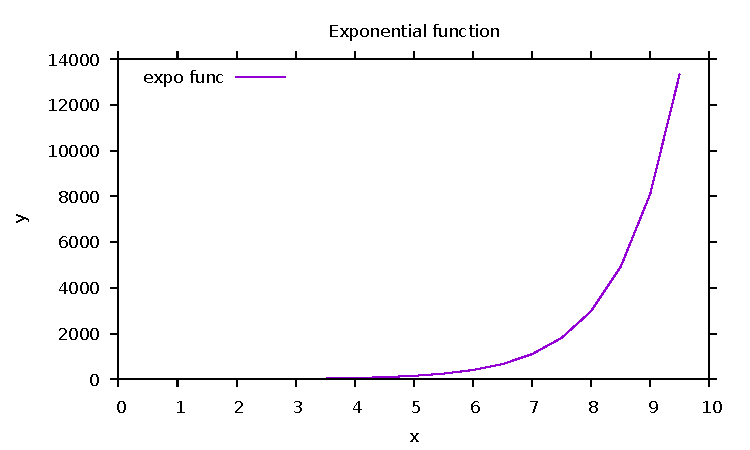
\includegraphics[width=\textwidth]{exp1.pdf}
    \caption{a nice plot}
    \label{fig:exp}
\end{figure}


The exponential function is one of the most important functions in mathematics (though it would have to admit that the linear function ranks even higher in importance). To form an exponential function, we let the independent variable be the exponent. A simple example is the functionThe exponential function is one of the most important functions in mathematics (though it would have to admit that the linear function ranks even higher in importance). To form an exponential function, we let the independent variable be the exponent. A simple example is the function:
The function seen in figure \ref{fig:exp} here is something that looks like: 
\begin{align}
e^x=\sum^{\infty}_{n=0} \frac{x^n}{n!} \label{Taylor_exp} \; . 
\end{align}
This function is widely used in both maths and physics to describer diverse functions and natural behaviours. 



\end{document}

